\section{Introduction}
\label{sect:intro}  % \label{} allows reference to this 
\subsection{Astrophysical Motivation}

High-contrast imaging instruments have been deployed on the ground (e.g. SCExAO\cite{Lozi18}, MagAO-X\cite{Males18}) and in space (e.g. NICMOS\cite{thompson_nicmos_1994}, NIRCam\cite{horner_nircam_2004}) to pursue the direct detection of extrasolar planets and exozodiacal dust. 
The Astro2020 Decadal Survey has identified that pursuing these instruments for the next generation of observatories is a key priority for the progression of astrophysical sciences\cite{Astro2020}. 
Currently there exists a gap between the theoretical limit on coronagraph performance and what modern realizations of these instruments are actually able to achieve. 
This is in part due to the sensitivity of coronagraphs to low-order aberrations minimizing the raw contrast achievable near the inner working angle (IWA)\cite{shaklan19}. 
We hypothesize that this performance gap can be spanned by providing a better connection between the ray trace model of the observatory and the wave propagation model of the coronagraph. 

Integrated models of optical observatories are highly beneficial to their use and design\cite{anderson_integrated_2011}. Open-source packages in particular have been widely used to simulate the performance of high-contrast imaging instrumentation. Tiny Tim was one of the first of these widely-used packages used to simulate the Hubble Space Telescope (HST)  instrument point-spread functions (PSF)\cite{Krist93}. The tool generates aberrated PSFs based on the instrument, observation, and dynamic aberrations for a given observing scenario, enabling highly accurate simulations of the observatory performance. However, this tool only considered aberrations that were conjugate to the exit pupil of the observatory. This limits the model's ability to capture out-of-pupil effects, like the Talbot effect and speckle from optical surfaces.
 To provide integrated modeling capabilities to future observatories, tools like PROPER \cite{Krist07}, POPPY\cite{Doug18}, and HCIPy \cite{por2018hcipy} were developed. These PSF simulation packages further integrated optical models of observatories by adding Fresnel diffraction to the PSF simulation, enabling the modeling of plane-to-plane diffraction effects. Near-field diffraction effects that limited high-contrast imaging could be modeled, and novel focal-plane wavefront sensing methods could be tested. FALCO\cite{Riggs18} is a similar tool that uses the same propagation physics to aid the design of these instruments by optimizing the commands sent to a deformable mirror to correct for the near-field diffraction effects that could limit the Roman Coronagraph's Sensitivity. These open-source physical optics propagation tools form the cornerstone of high-contrast imaging instrument modeling and design, but they do not exist in a vacuum. To account for effects that aren't traceable through the assumptions made by Fresnel diffraction, these models must be linked to other software.
Presently the optical design of observatories are done in a ray-tracing engine (e.g. CODE V, OpticStudio) because it is more suitable to optimizing the shapes of observatory mirrors. Upon reaching a diffraction-limited optical design, the system is then assumed to be well-represented by a paraxial diffraction model. The wavefront maps produced by the ray trace model of the observatory and the contributions from the imperfect polishing of the observatory mirrors are sent to an open-source physical optics code (e.g. PROPER, POPPY, HCIPy) to examine the image plane field in the presence of diffraction from structure in the beam and phase errors on the optics. 

\begin{table}[H]
    \centering
    \begin{tabular}{c c c c}
        \hline
        Design Code & Ray Trace & Wave Propagation & Open Source \\
        \hline
        CODE V & \checkmark & \checkmark & \\
        OpticStudio & \checkmark & \checkmark  & \\
        FRED & \checkmark & \checkmark  & \\
        POPPY & & \checkmark & \checkmark  \\
        HCIPy & & \checkmark & \checkmark \\
        PROPER & & \checkmark & \checkmark \\
        \hline
        \\
    \end{tabular}
    \caption{Comparison of commonly-used software's ability to ray trace, do physical optics, and be open source. Consider replacing with a table.}
    \label{tab:design_software_compare}
\end{table}

While this approach has been suitable to the modeling of an instrument's PSF, it is less integrated, and makes the assumption that the optical field is well-represented by Fresnel diffraction. Commercial optical design codes offer the ability to make diffraction calculations based on ray data, but their physical optics simulation techniques aren't as transparent or versatile as the open-source propagation codes that are used to design coronagraphs for astronomical observatories. The current open-source physical optics codes used for observatory modeling are also limited in their scope because of the Fresnel approximation, which is incapable of accurately modeling the field after fast-focusing surfaces, highly aspheric\cite{krist_practical_2010} surfaces, and non-uniform pupils\cite{vanderbei_diffraction_2006}. As observatories get larger, their optics must become faster and more aspheric to fit within a reasonable volume. Some coronagraph architectures capable of earthlike exoplanet detection (e.g. PIAA\cite{guyon_phase_nodate}) employ mirrors that apodize the pupil with highly aspheric mirrors, and require tailored propagators in order to be included in physical optics models\cite{krist_practical_2010}. In the regime where the contribution of these surfaces is best represented by a ray trace, a diffraction calculation must be made to appropriately model the optical field at the image plane.


%The Structural- Thermal- Optical-Performance (STOP) modeling flow for the Roman Coronagraph Instrument (Roman-CGI), for example, relies on multiple proprietary software packages in order to simulate the coronagraphic point-spread function (PSF). First Thermal Desktop is used to determine the temperature field across the observatory. These data are sent to NASTRAN to compute the structural deformations in the observatory. This is then translated to the CODE V model of the observatory through SIGFIT so that they wavefront error can be output as a series of Zernike polynomials.  The wavefront error decomposition is then propagated through PROPER, an open-source  physical optics library, to simulate the wavefront sensing, control, and final image field \cite{Krist18}. While effective, we believe that this process can be further integrated using insights from optical physics to simplify and open-source the propagation of the optical field.

\begin{figure}[H]
	\centering
	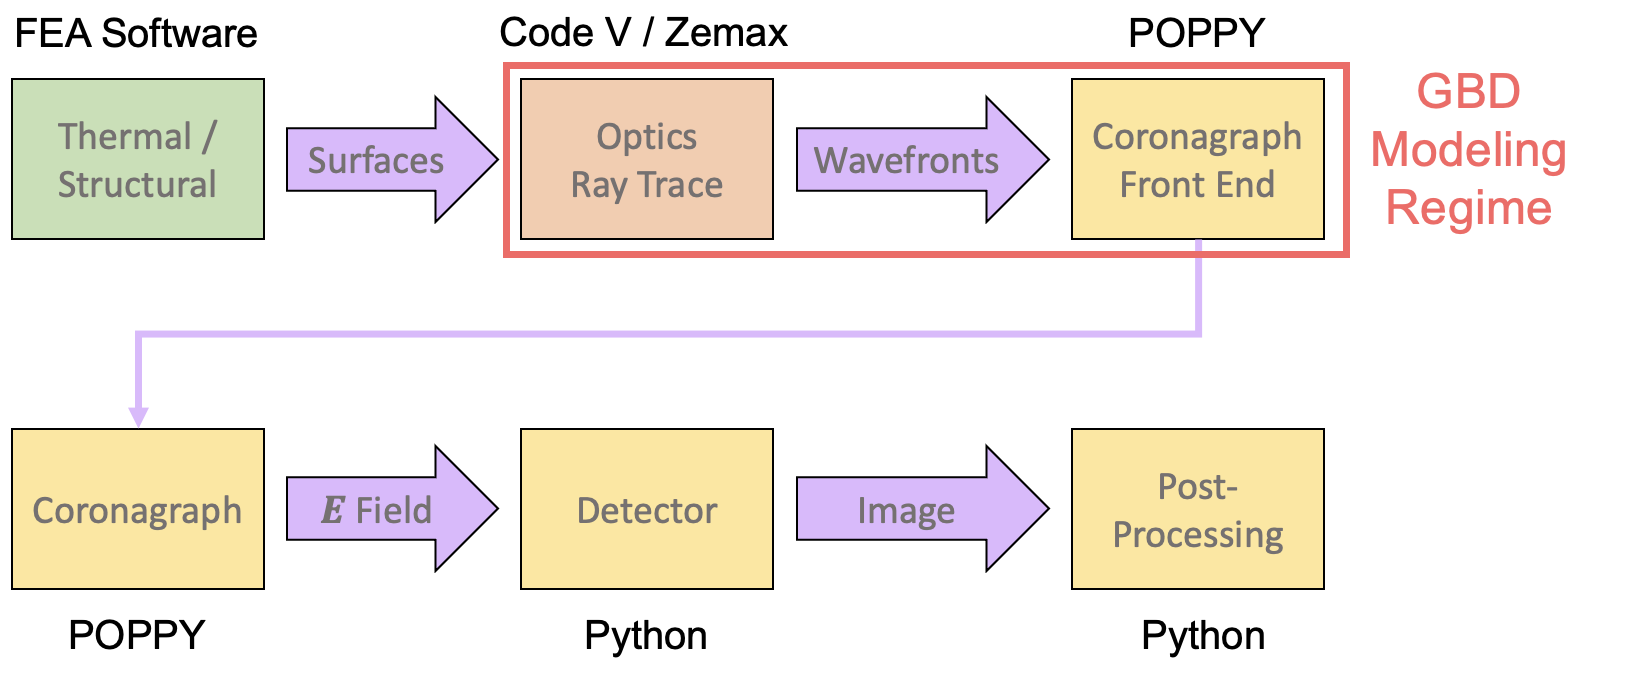
\includegraphics[width=\textwidth]{stop_flow.png}
	\caption{Modeling flow inspired by the STOP modeling process for Roman Coronagraph \cite{Krist18}. This diagram illustrates the different software packages and their associated modeling regimes. The dashed red box shows the region that could be unified using Gaussian Beamlet Decomposition as a propagation technique, which would open-source the ray-based physical optics of ray tracing codes.}
\end{figure} 

To bridge the gap between commercial ray tracing engines and open-source physical optics propagation codes we investigate the viability of a ray-based diffraction calculation for designing observatories with coronagraphs called Gaussian Beamlet Decomposition (GBD). The technique has been previously implemented in commercial codes (CODE V\cite{StoneTechMemo}, FRED\cite{FredTechMemo}) and been recently developed to improve its viability for precision diffraction simulation \cite{Worku17,Worku:18,Worku19}. However, the method has not seen wide implementation in the world of open-source physical optics propagators, and has not yet been formally evaluated as a tool to augment the modeling of observatories equipped with high-contrast imaging instrumentation. 

\subsection{Gaussian Beamlet Decomposition}

Gaussian Beamlet Decomposition (GBD) is a method of physical optics propagation that approximates the propagated field as a finite sum of Gaussian beams. This method has been implemented in many optical design packages \cite{greynolds_ten_2020} to perform coherent calculations on non-paraxial systems. Fourier transform-based propagation methods derived from the Huygens-Fresnel diffraction integral typically assume the field is scalar and optical system is paraxial \cite{goodman17}. This is a fair assumption for astronomical coronagraphs which operate on slowly focusing beams with diffraction-limited optics. Astronomical observatories however, employ fast mirrors with conic surfaces to collect a large amount of light in a relatively short instrumental volume. Observatories are designed and modeled in ray trace software to accurately model the wavefront in the exit pupil. Upon finalizing the design, the complex exit pupil is sent to a Fourier-based physical optics propagator to simulate the performance of a high-contrast imaging instrument. GBD aims to compute the same complex optical field without making the paraxial assumption across the instrument. Rather, the propagation of a generally astigmatic Gaussian beam is derived from the Collins integral\cite{collins,cai_decentered_nodate} which imposes the paraxial assumption about a single Gaussian beamlet, which is a much less stringent approximation. Gaussian's are technically infinite in extent, but 99$\%$ of the energy is enclosed within the $~ 2/e$ irradiance radius. Consequently, the contribution of the field very far from the Gaussian is negligible. This parameter enables the optical system to generally be non-paraxial, providing that the beamlets are not very divergent\cite{Harvey15}.

\subsection{Hybrid Propagation Physics}

The ray-based nature of GBD introduces problems in modeling the electric field when the rays are vignetted. For a Lyot-type coronagraph all rays are vignetted at the focal plane mask which eliminates the field decomposition. To circumvent this we compute the field before the focal plane mask with GBD and propagate it through the remaining coronagraph with Fresnel diffraction. This \emph{hybrid} method enables the user to alter the propagation physics for the electric field based on where it is the most appropriate.

\begin{figure}[H]
    \centering
    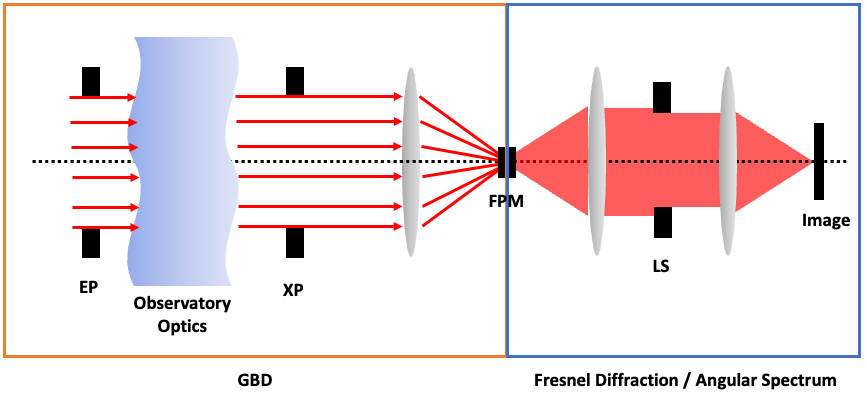
\includegraphics[width=\textwidth]{hybridpropdiagram.png}
    \caption{Diagram demonstrating the hybrid propagation physics model. The observatory optics are best described by a ray-based propagation model, so GBD is used to compute the field at the image plane before the coronagraph FPM. The field array is then handed to a Fresnel propagation model which propagates it past the FPM and through the remainder of the coronagraph.}
    \label{fig:hybridpropdiagram}
\end{figure}

The end result of such a model allows for direct integration of the ray trace model with the physical optics model, without imposing the paraxial approximation on the observatory. Like Fresnel, GBD is an approximation to diffraction physics. The decomposition of the field into gaussian beams does not have a unique solution. Therefore, undesirable artifacts can be introduced into the field if the decomposition is not well-understood and the sampling is insufficient\cite{Ashcraft2020}. To better understand the impact of a GBD PSF on high-contrast imaging simulations, we develop a hybrid propagation model to compare GBD to an equivalent Fresnel diffraction model.  In section 2 we outline the mathematics of the Gaussian Beam and how it is used to simulate an observatory PSF. In section 3 we compare the results of observatory PSFs produced by GBD with one produced using traditional Fourier transform-based diffraction methods. In section 4 we assess the suitability of GBD for high-contrast imaging models and establish a roadmap for our module's development.

% Traditional diffraction modeling regimes consider the optical system to be paraxial and the electromagnetic field to be essentially scalar. Gaussian Beamlet Decomposition (GBD) is a ray-based method of diffraction calculation that approximates an optical field as a superposition of Gaussian beams. Gaussian beams are unique in that they can be propagated along ray paths. In their seminal paper, Harvey et al\cite{Harvey15} reviews the theory of complex ray tracing used to propagate Gaussian beams. 
